\section{Running COMPSs applications}
\label{sec:RunningApps}

\subsection{Compiling and Packaging the application}
\label{subsec:compiling_and_packaging_apps}

The application can be compiled either using the command line or through the Eclipse IDE tool available on the SDK VM.

\begin{lstlisting}[language=bash]
user@bsccompss:~$ cd /home/user/workspace/
user@bsccompss:~/workspace$ javac simple/src/simple/*.java
user@bsccompss:~/workspace/simple/src$ jar cf simple.jar simple 
\end{lstlisting}


Once the application is compiled and packaged in a {\bf Jar archive} it have to be bundled in a {\bf tar.gz} package; 
this package will be automatically deployed by COMPSs in a cloud environment, while in the case of a static pool of 
physical nodes the jar has to be manually pre-deployed.

In this example the application package is stored under {\bf /home/user/workspace/APPNAME/package}

\begin{lstlisting}[language=bash]
user@bsccompss:~/workspace/simple/src$ tar czvf Simple.tar.gz simple.jar
user@bsccompss:~/workspace/simple/src$ mv Simple.tar.gz ~/workspace/simple/package/
\end{lstlisting}

In case of having to supply external binaries or libraries to the application, as is the case of Blast 
(see Section \ref{sec:SampleApps}) they have to be copied into a directory named ``binary'', and ``lib''
respectively and packaged in the {\bf tar.gz} package as shown below:

\begin{figure}[h!]
  \centering
    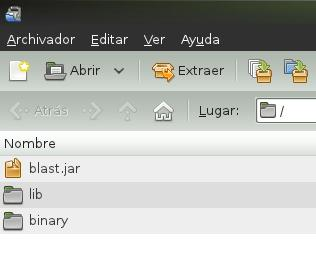
\includegraphics[width=60mm]{./Sections/3_Running_Apps/Figures/example_package.jpeg}
    \caption{An example package. \label{fig:example_package}}
\end{figure}



\subsection{Running the application}
\label{subsec:running_apps}

To run the application on the SDK VM, the path of the application jar must be added to {\bf CLASSPATH} system variable:

\begin{lstlisting}[language=bash]
user@bsccompss:~$ cp ~/workspace/simple/package/Simple.tar.gz   /home/user/
user@bsccompss:~$ tar xzf Simple.tar.gz
user@bsccompss:~$ export CLASSPATH=$CLASSPATH:/home/user/simple.jar
\end{lstlisting}

Once the execution environment is ready, the application can be launched through the following command:

\begin{lstlisting}[language=bash]
user@bsccompss:~$ runcompss simple.Simple <initial_number>
\end{lstlisting}

\begin{figure}[h!]
  \centering
    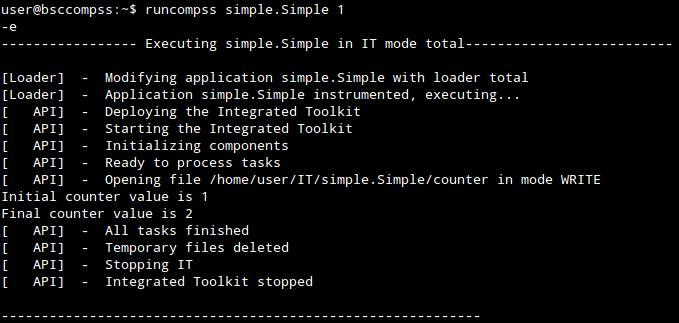
\includegraphics[width=0.95\textwidth]{./Sections/3_Running_Apps/Figures/compss_execution.jpeg}
    \caption{Execution of a COMPSs application. \label{fig:compss_execution}}
\end{figure}
\vspace{-0.4cm}


\subsection{Logging the execution}
The {\bf it.log} file, that can be found generally in {\bf \$HOME/it.log} ({\bf /home/user/it.log, in case of SDK VM}). 
It shows information on the execution of the application including file transfers and job submission details.

\begin{lstlisting}[language=bash]
user@bsccompss:~$ tail -f it.log
\end{lstlisting}

On the other hand, the {\bf resources.log} file, that can be found in {\bf \$HOME/resources.log}. It shows information 
about the available resources such as: number of processors of each resource (slots), information about running or 
pending tasks in the resource queue as depicted in the following picture:

\begin{figure}[h!]
  \centering
    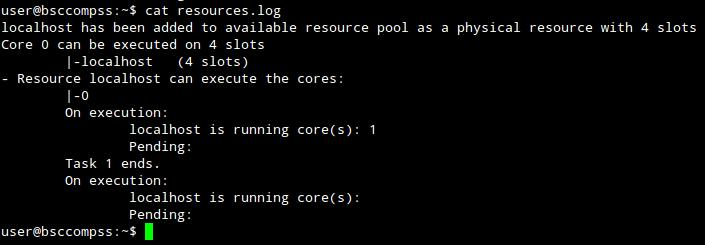
\includegraphics[width=0.95\textwidth]{./Sections/3_Running_Apps/Figures/available_resources.jpeg}
    \caption{Information on the available resources. \label{fig:available_resources}}
\end{figure}


\subsection{Execution results}
After the execution, COMPSs stores the files corresponding to the {\bf stdout} and {\bf stderr} of each task in the 
{\bf /home/user/IT/APPNAME/} directory.

\begin{figure}[h!]
  \centering
    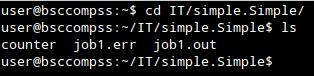
\includegraphics[width=0.6\textwidth]{./Sections/3_Running_Apps/Figures/task_log1.jpeg}
    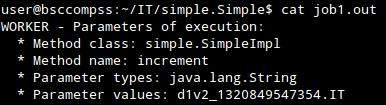
\includegraphics[width=0.6\textwidth]{./Sections/3_Running_Apps/Figures/task_log2.jpeg}
    \caption{The log of each task can be retrieved at the end of the execution. \label{fig:task_logs}}
\end{figure}

The results of an execution will be stored in the {\bf /home/user/IT/simple.Simple/} directory in the example application.


\subsection{Exploring the final execution graph}
At the end of the execution a dependency graph can be generated representing the order of execution of each type of 
task and their dependencies.

\begin{lstlisting}[language=bash]
user@bsccompss:~$ gengraph graph.dot
\end{lstlisting}

\begin{figure}[h!]
  \centering
    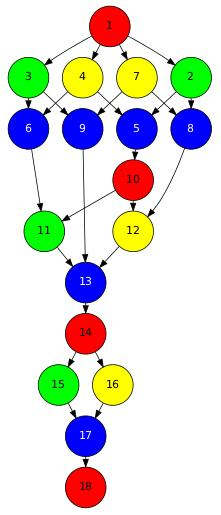
\includegraphics[width=0.3\textwidth]{./Sections/3_Running_Apps/Figures/dependency_graph.jpeg}
    \caption{The dependency graph of the SparseLU application. \label{fig:dependency_graph}}
\end{figure}

\subsection{COMPSs monitoring system}
The COMPSs runtime exposes a Web Service with a graphical interface that can be used to monitor the progress of running 
applications. In order to see it, a specific URL must be used in a web browser:

\begin{lstlisting}[language=bash]
http://localhost:8080/compss-monitor
\end{lstlisting}

As it can be seen in Figure \ref{fig:monitoring_interface}, the interface gives details about the execution graph 
(it can be seen how the data dependency graph is built and consumed at real time, and the status of the tasks), 
the resource usage information, the number of tasks, and the execution time per task.

\begin{figure}[thb!]
  \centering
    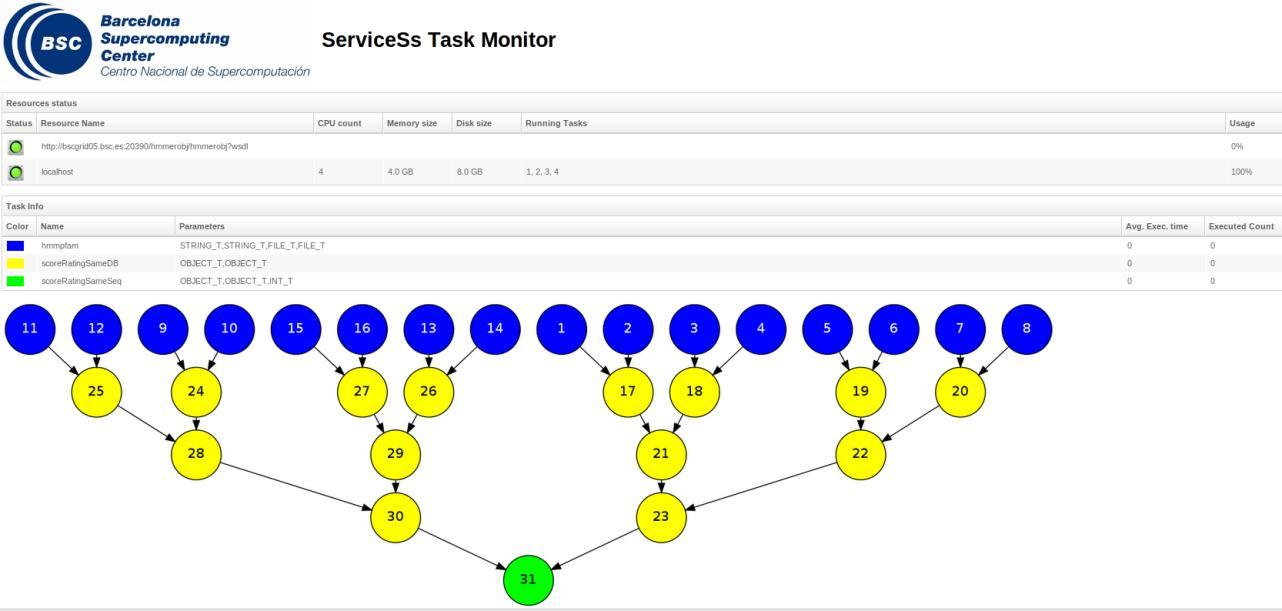
\includegraphics[width=0.9\textwidth]{./Sections/3_Running_Apps/Figures/compss_monitoring.jpeg}
    \caption{COMPSs monitoring interface example. \label{fig:monitoring_interface}}
\end{figure}